\documentclass[reprint,amsmath,amssymb,aps,showkeys,superscriptaddress]{revtex4-2}

\usepackage{graphicx}
\usepackage{dcolumn}
\usepackage{bm}% bold math
\usepackage{braket}
\usepackage{xcolor}
\newcommand{\red}{\textcolor{red}}
\newcommand{\blue}{\textcolor{blue}}
\newcommand{\magenta}{\textcolor{magenta}}
\newcommand{\green}{\textcolor{green}}
\begin{document}

\title{Particle Dynamics in Digital Black-Hole Spacetimes}

\author{Yuki Matsuno}
 \affiliation{Department of Physics, College of Humanities and Sciences, Nihon University, Sakura-josui,
 Tokyo 156-8550, Japan}
\author{Shunichiro Kinoshita}
 \email{kinoshita@neptune.kanazawa-it.ac.jp}
 \affiliation{Mathematics, Science, Data Science and AI Program, Kanazawa Institute of Technology, Nonoichi, Ishikawa 921-8501, Japan} 
 \author{Keiju Murata}
 \email{murata.keiju@nihon-u.ac.jp}
  \affiliation{Department of Physics, College of Humanities and Sciences, Nihon University, Sakura-josui,
 Tokyo 156-8550, Japan}
 \affiliation{Global R\&D Center for Business by Quantum-AI Technology (G-QuAT),
National Institute of Advanced Industrial Science and Technology (AIST),
1-1-1 Umezono, Tsukuba, Ibaraki 305-8568, Japan}
 \author{Daisuke Yamamoto}
 \email{yamamoto.daisuke21@nihon-u.ac.jp}
 \affiliation{Department of Physics, College of Humanities and Sciences, Nihon University, Sakura-josui,
 Tokyo 156-8550, Japan}
\affiliation{Global R\&D Center for Business by Quantum-AI Technology (G-QuAT),
National Institute of Advanced Industrial Science and Technology (AIST),
1-1-1 Umezono, Tsukuba, Ibaraki 305-8568, Japan}
\affiliation{RIKEN Center for Quantum Computing (RQC), Wako, Saitama 351-0198, Japan}

\begin{abstract}
We study particle dynamics in a one-dimensional lattice Majorana-fermion model designed to emulate black-hole and white-hole spacetimes. By encoding the effective metric into position-dependent lattice couplings, we analyze the low-momentum dispersion relation and the associated effective light-cone structure. Using real-space Bogoliubov--de Gennes diagonalization and wave-packet time evolution, we show that packet trajectories agree with the corresponding geodesic motion for black-hole profiles. We also extract the surface gravity from the near-horizon growth of the wave-packet standard deviation and compare the numerical result with the analytical scaling. For the white-hole geometry, we show that wave-packet compression leads to finite-size reflection, with a stagnation time that scales logarithmically with the system size. We further clarify lattice-specific effects, including doubler-induced oscillations inside the black hole and partial transmission in the white-hole geometry. These results support lattice fermion models as practical platforms for quantum simulation of black-hole spacetime particle dynamics while clarifying the lattice artifacts that limit their range of validity.
\end{abstract}

\maketitle

\section{INTRODUCTION}
Quantum simulation provides a route to realizing and probing quantum theories by encoding their dynamics in controllable many-body systems \cite{Feynman1982,Lloyd1996}. A particularly compelling target is quantum field theory (QFT) in curved spacetime, which describes quantum fields propagating on prescribed gravitational backgrounds and predicts fundamental phenomena such as cosmological particle creation, the Unruh effect, and Hawking radiation \cite{Parker1968,Parker1969,Unruh1976,Hawking1975}. These phenomena lie at the interface of quantum theory and gravitation, yet their direct observation remains exceptionally challenging. This has motivated the development of experimentally accessible platforms in which curved-spacetime QFTs and their characteristic dynamics can be investigated under controlled conditions.

A major route toward this goal has been analog gravity, pioneered by Unruh’s demonstration that sound waves in a transonic fluid obey equations equivalent to those of a field near a black-hole horizon \cite{Unruh1981}. This idea has developed into a broad research program in which collective excitations in engineered media, such as phonons in Bose--Einstein condensates and electromagnetic waves in nonlinear optical systems, experience an emergent effective metric, typically within a hydrodynamic or long-wavelength regime \cite{Barcelo2011,Garay2000,Lahav2010,Philbin2008}. Such platforms have provided powerful laboratory access to horizon physics and the associated wave-conversion phenomena. Their curved geometry, however, is an effective description of excitations supported by the host medium and is consequently tied to its microscopic dynamics and dispersive corrections, rather than arising from a direct discretization of a prescribed curved-spacetime QFT.

A conceptually distinct route is to discretize a prescribed curved-spacetime QFT itself so that the target theory is recovered in a controlled continuum limit. Quantum-walk and lattice approaches have pursued this direction by encoding geometry into discrete dynamics or spatially inhomogeneous local couplings \cite{DiMolfetta2013,Yang2020,LewisVidal2020}. In previous work by some of us, a general correspondence was established between Majorana QFTs in arbitrary $(1+1)$-dimensional curved spacetimes with periodic spatial topology and one-dimensional spin-$1/2$ systems, with the metric mapped directly onto space- and time-dependent exchange couplings and magnetic fields \cite{Kinoshita2025}. We refer to this framework, and more generally to such controlled lattice encodings of prescribed curved-spacetime QFTs, as \emph{digital curved spacetimes}. Here, ``digital'' primarily denotes the spatial discretization of the field theory itself, rather than any specific gate-based protocol, while also reflecting the natural compatibility of the resulting local lattice Hamiltonians with digital quantum processors and other programmable quantum-simulation platforms \cite{Altman2021}. The framework has subsequently been applied to thermal detector responses in an inflationary spacetime and extended to QFTs with spatial boundaries \cite{KinoshitaInflation2025,KinoshitaBoundary2026}. Unlike in analog-gravity platforms, the geometry is imposed through an explicit metric-to-coupling dictionary, and the target continuum theory is recovered systematically as the lattice spacing is reduced.

Black-hole spacetimes provide a particularly stringent test of such lattice encodings. Position-dependent hopping and spin models have been used to study transport, entanglement, and information transfer near nominal lattice horizons, with outward propagation interpreted in some works as stimulated Hawking radiation or information escape \cite{Yang2020,Shi2023,Benhemou2023,Liu2026}. Before making such an interpretation, however, one must first verify that the lattice model reproduces the elementary causal dynamics of the target continuum QFT. A pre-existing one-particle wave packet initially inside a future horizon must propagate further into the black-hole interior rather than return to the exterior, whereas Hawking radiation, when present, is a distinct quantum-field-theoretic particle-production process. Establishing this basic correspondence and quantifying its finite-lattice corrections are therefore essential prerequisites for using lattice models to address genuinely quantum horizon phenomena.


In this work, we establish this correspondence for particle dynamics in digital black-hole spacetimes. Starting from a one-dimensional lattice Majorana model obtained through the metric-to-coupling correspondence~\cite{Kinoshita2025}, we demonstrate that localized wave packets quantitatively follow the corresponding continuum geodesics as the lattice spacing is reduced. In particular, wave packets initialized inside a future horizon propagate further into the black-hole interior, faithfully reproducing its one-way causal structure. We further show that the surface gravity can be extracted from the evolution of the wave-packet width, and clarify how finite-size effects, fermion doubling, and different lattice regularizations modify the approach to the continuum limit. By contrasting black-hole and white-hole geometries, we separate the universal causal dynamics of the target spacetime from regularization-dependent lattice effects. These results establish a controlled benchmark for digital curved spacetimes and provide a necessary foundation for their extension to intrinsically quantum horizon phenomena, including Hawking particle production and quantum-information transport, as well as to time-dependent geometries and implementations on programmable quantum processors.

%{This paper is organized as follows. In Sec. II, we introduce the one-dimensional lattice fermion model and explain how the effective metric and horizon structure emerge from its low-momentum dispersion. In Sec. III, we study wave-packet dynamics in a black-hole profile, compare the resulting trajectories with the corresponding geodesics, and analyze the role of fermion doubling. We also extract the surface gravity from wave-packet broadening and then examine finite-size effects in a white-hole profile. Finally, Sec. IV summarizes our results and discusses future directions.}

%Throughout this paper, we use natural units with $\hbar=c=1$.

\section{Digital black-hole spacetime on a lattice}
\label{sec:model}

We consider a massless Majorana field in a static
$(1+1)$-dimensional curved spacetime described by the
Painlev\'e--Gullstrand-type metric
\begin{equation}
  ds^2
  =
  -\bigl[1-\beta^2(x)\bigr]dt^2
  -2\beta(x)\,dt\,dx
  +dx^2.
  \label{eq:PG_metric}
\end{equation}
This coordinate system is regular at the horizon and covers the
exterior and interior regions within a single time slicing, allowing
particle propagation across the horizon to be followed without
encountering a coordinate singularity. A horizon is located at
$x=x_{\mathrm h}$ satisfying
\begin{equation}
  \bigl|\beta(x_{\mathrm h})\bigr|=1.
  \label{eq:horizon_condition}
\end{equation}
The Hamiltonian of the massless Majorana field on this background is
\begin{equation}
\begin{aligned}
  H_{\mathrm{QFT}}
  =
  \int_0^\ell dx\,
  \Bigl[
  &-\frac{1}{2}
  \left(
    \phi^\dagger\partial_x\phi^\dagger
    -
    \phi\partial_x\phi
  \right)
  \\
  &-\frac{i\beta(x)}{2}
  \left(
    \phi^\dagger\partial_x\phi
    +
    \phi\partial_x\phi^\dagger
  \right)
  \Bigr],
\end{aligned}
  \label{eq:continuum_Hamiltonian}
\end{equation}
where $\ell$ is the length of the spatial interval. The field
operators satisfy the equal-time canonical anticommutation relation
\begin{equation}
  \left\{
    \phi(t,x),\phi^{\dagger}(t,y)
  \right\}
  =
  \delta(x-y),
\label{eq:continuum_anticommutation}
\end{equation}
with all other anticommutators vanishing.

The field-to-spin dictionary developed in
Ref.~\cite{Kinoshita2025} is characterized by five space- and
time-dependent functions. The three functions
$\alpha(t,x)$, $\beta(t,x)$, and $\gamma(t,x)$ determine the
spacetime metric, $\zeta(t,x)$ specifies a local gauge choice for the
Majorana field, and $p(t,x)$ parametrizes a nontrivial freedom in the
spin-lattice realization. To obtain the static
Painlev\'e--Gullstrand geometry in Eq.~\eqref{eq:PG_metric}, we set
\begin{equation}
  \alpha(t,x)=\gamma(t,x)=1,
  \qquad
  \beta(t,x)=\beta(x).
  \label{eq:dictionary_specialization}
\end{equation}
We also fix the gauge as $\zeta(t,x)=0$ and, for simplicity, restrict
$p(t,x)$ to a spatially and temporally uniform constant $p$. 
Under this specialization, the dictionary maps the Majorana QFT on
the Painlev\'e--Gullstrand background onto the
Majorana QFT onto an anisotropic $XY$ chain with a bond-dependent Dzyaloshinskii--Moriya interaction and a transverse field:
\begin{align}
  H_{\mathrm{spin}}
  ={}&
  -\frac{1}{4\varepsilon}
  \sum_{j=1}^{L-1}
  \Bigl[
    (1+p)\sigma_j^x\sigma_{j+1}^x
    -(1-p)\sigma_j^y\sigma_{j+1}^y
  \nonumber\\
  &\hspace{18mm}
    -\beta_{j+1/2}
    \left(
      \sigma_j^x\sigma_{j+1}^y
      -
      \sigma_j^y\sigma_{j+1}^x
    \right)
  \Bigr]
  \nonumber\\
  &-\frac{p}{2\varepsilon}
  \sum_{j=1}^{L}\sigma_j^z.
  \label{eq:spin_Hamiltonian}
\end{align}


The shift function $\beta(x)$, which specifies the spacetime geometry, is encoded in the bond-dependent
Dzyaloshinskii--Moriya coupling. Here, we evaluate the shift function at the center of each bond,
\begin{equation}
  \beta_{j+\frac12}
  \equiv
  \beta\left(x_{j+\frac12}\right),
  \qquad
  x_{j+\frac12}
  =
  \varepsilon\left(j+\frac12\right).
  \label{eq:lattice_beta}
\end{equation}
This bond-centered convention aligns the sampling point of
$\beta(x)$ with the spatial location of the
Dzyaloshinskii--Moriya coupling that it determines. It differs from
the site-centered convention
$\beta_j=\beta(x_j)$ adopted in Ref.~\cite{Kinoshita2025} only at
finite lattice spacing, and the two prescriptions yield the same
continuum QFT as $\varepsilon\to0$.

For the analytical and numerical treatment below, we rewrite the
spin Hamiltonian in terms of Jordan--Wigner fermions. For a finite
open chain, this gives
\begin{align}
  H
  ={}&
  -\frac{1}{2\varepsilon}
  \sum_{j=1}^{L-1}
  \Bigg[
    c_{j+1}c_j
    +
    c_j^\dagger c_{j+1}^\dagger
    +
    p\left(
      c_j^\dagger c_{j+1}
      +
      c_{j+1}^\dagger c_j
    \right)
  \nonumber\\
  &\hspace{10mm}
    +
    i\beta_{j+\frac12}
    \left(
      c_j^\dagger c_{j+1}
      -
      c_{j+1}^\dagger c_j
    \right)
  \Bigg]
  \nonumber\\
  &-
  \frac{p}{2\varepsilon}
  \sum_{j=1}^{L}
  \left(
    1-2c_j^\dagger c_j
  \right).
  \label{eq:lattice_Hamiltonian}
\end{align}
The operators satisfy
\begin{equation}
  \{c_j,c_{j'}^\dagger\}
  =
  \delta_{jj'},
  \label{eq:lattice_anticommutation}
\end{equation}
with all other anticommutators vanishing.

As established in Ref.~\cite{Kinoshita2025}, this Jordan--Wigner
representation is related to the continuum Majorana field through
the spatial discretization
\begin{equation}
  c_j
  =
  \sqrt{\varepsilon}\,
  \phi(x_j),
  \qquad
  x_j=\varepsilon j,
  \label{eq:continuum_identification}
\end{equation}
with the continuum theory recovered as
$\varepsilon\to0$ at fixed physical length
$\ell=\varepsilon L$. Thus,
Eq.~\eqref{eq:lattice_Hamiltonian} is simultaneously the exact
fermionic representation of the local spin simulator and a
controlled lattice realization of the target curved-spacetime QFT.

As shown in Ref.~\cite{KinoshitaBoundary2026}, the function
$p(t,x)$ has two distinct roles in the field-to-spin dictionary.
First, it participates in the realization of spatial boundary
conditions in a finite open chain. Second, it controls the
ultraviolet structure of the bulk lattice theory, including the
presence and momentum-space structure of fermion doublers, without
modifying the target spacetime geometry or continuum QFT. In the
present work, the horizon and the initial wave packets are placed
sufficiently far from the physical ends of the chain that boundary
effects are negligible over the time scales considered. We therefore
restrict $p(t,x)$ to the constant choices
\begin{equation}
  p=0
  \qquad\text{and}\qquad
  p=1,
  \label{eq:p_choices}
\end{equation}
and focus on its second role, namely the regularization-dependent
bulk dynamics.


\subsection{Local dispersion and causal velocities}
\label{subsec:dispersion}

To identify the bulk modes relevant to the wave-packet dynamics, we
examine the local dispersion relation of the lattice model. Since
$\beta(x)$ varies in space, momentum is not a good quantum number for
the full open chain. We therefore consider an auxiliary homogeneous
chain of $L'$ sites in which $\beta(x)$ is replaced by a constant
local value $\beta$ and periodic boundary conditions are imposed.
Here, $L'$ denotes the number of sites in this auxiliary homogeneous
system and is distinct from the size $L$ of the open chain used in
the real-space simulations.

Using the Fourier transformation
\begin{equation}
  c_j
  =
  \frac{1}{\sqrt{L'}}
  \sum_{\kappa}
  e^{i\kappa j}c_{\kappa},
  \qquad
  \kappa=\frac{2\pi n}{L'},
  \label{eq:Fourier_transform}
\end{equation}
where $\kappa\in[-\pi,\pi)$ is the dimensionless lattice momentum,
the homogeneous Hamiltonian can be written in the
Bogoliubov--de Gennes form
\begin{equation}
  H
  =
  \frac{1}{2}
  \sum_{\kappa}
  \Psi_{\kappa}^{\dagger}
  \mathcal{H}(\kappa)
  \Psi_{\kappa}
  +\mathrm{const.},
  \label{eq:BdG_Hamiltonian}
\end{equation}
where
\begin{equation}
  \Psi_{\kappa}
  =
  \begin{pmatrix}
    c_{\kappa}\\
    c_{-\kappa}^{\dagger}
  \end{pmatrix},
  \label{eq:Nambu_spinor}
\end{equation}
and
\begin{equation}
  \mathcal{H}(\kappa)
  =
  \frac{1}{\epsilon}
  \begin{pmatrix}
    \beta\sin\kappa
    +p(1-\cos\kappa)
      & -i\sin\kappa
    \\
    i\sin\kappa
      & \beta\sin\kappa
        -p(1-\cos\kappa)
  \end{pmatrix}.
  \label{eq:BdG_matrix}
\end{equation}
The two eigenvalue branches are
\begin{equation}
\begin{aligned}
  E_{\pm}(\kappa)
  =
  \frac{1}{\epsilon}
  \Biggl[
    \beta\sin\kappa
    \mathbin{\pm}
    \Bigl\{
      \sin^{2}\kappa
      +p^{2}(1-\cos\kappa)^{2}
    \Bigr\}^{1/2}
  \Biggr].
\end{aligned}
  \label{eq:lattice_dispersion}
\end{equation}

To take the continuum limit, we introduce the physical momentum
\begin{equation}
  k=\frac{\kappa}{\epsilon}
  \label{eq:physical_momentum}
\end{equation}
and let $\epsilon\to0$ at fixed $k$, so that
$\kappa=\epsilon k\to0$. The dispersion then becomes
\begin{equation}
  E_{\pm}(\epsilon k)
  =
  \beta k
  \pm |k|
  +O\!\left(\epsilon^{2}|k|^{3}\right).
  \label{eq:continuum_dispersion_general}
\end{equation}
For the positive-momentum sector, $k>0$, this reduces to
\begin{equation}
  E_{\pm}(\epsilon k)
  =
  (\beta\pm1)k
  +O\!\left(\epsilon^{2}k^{3}\right).
  \label{eq:continuum_dispersion}
\end{equation}
The corresponding physical group velocities are therefore
\begin{equation}
  v_{\pm}
  =
  \frac{\partial E_{\pm}}{\partial k}
  =
  \epsilon
  \frac{\partial E_{\pm}}{\partial\kappa}
  \longrightarrow
  \beta\pm1
  \qquad
  (\epsilon\to0).
  \label{eq:group_velocities}
\end{equation}
These coincide with the two null characteristic velocities of the
Painlev\'e--Gullstrand metric,
\begin{equation}
  \frac{dx}{dt}
  =
  \beta(x)\pm1,
  \label{eq:null_characteristics}
\end{equation}
obtained by setting $ds^{2}=0$.


\begin{figure}[t]
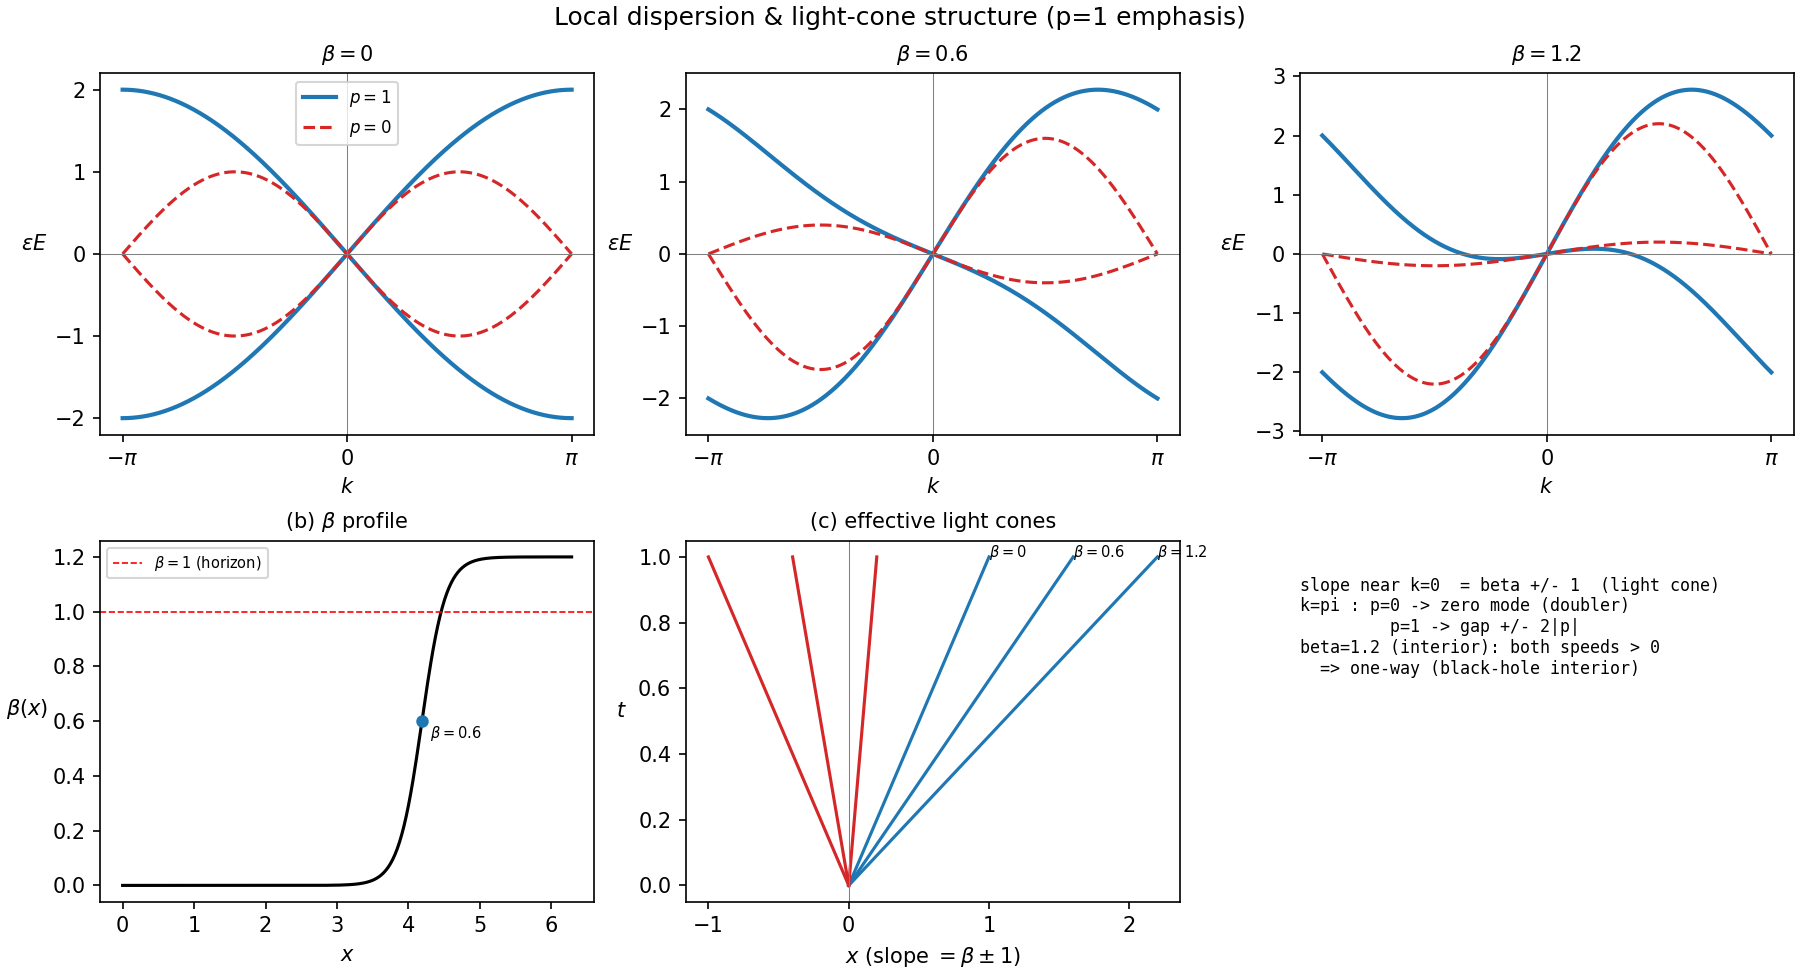
\includegraphics[width=\linewidth]{figure/dispersion.png}
\caption{
Local dispersion relations for (a) $p=0$ and (b) $p=1$ at
$\beta=0$, $1$, and $2$, shown from left to right.
(c) An example of the spatial profile $\beta(x)$ used in the real-space analysis. The dashed line marks $\beta=1$, where the horizon is located.
(d) Sketches of the corresponding local light cones determined by
the low-momentum group velocities. Inside the horizon, where $\beta>1$, both characteristic velocities
are positive and point toward the black-hole interior.
}
\label{fig:local_dispersion}
\end{figure}

The corresponding local dispersion relations are shown in
Figs.~\ref{fig:local_dispersion}(a) and
\ref{fig:local_dispersion}(b) for $p=0$ and $p=1$, respectively. The three columns correspond to $\beta=0$, $1$, and $2$.
For $\beta=0$, the two low-momentum branches have opposite group
velocities, $v_{\pm}=\pm1$.
At $\beta=1$, one of the characteristic velocities vanishes,
signaling the formation of a horizon.
For $\beta>1$, both low-momentum velocities become positive, and
hence both branches propagate toward increasing $x$.

Although the two choices of $p$ reproduce the same low-momentum
dispersion, their finite-momentum structures are qualitatively
different. For $p=0$, additional zero-energy modes occur at the
Brillouin-zone edges $\kappa=\pm\pi$, corresponding to conventional
fermion doublers. Their physical momenta are of order
$|k|\sim\pi/\epsilon$, even though their excitation energies remain
low. For $p>0$, the term $p(1-\cos\kappa)$ lifts the zero-energy modes at
the Brillouin-zone edges. Its momentum dependence is analogous to
that of the Wilson term introduced to remove fermion doublers in
lattice gauge theories \cite{Wilson1974}. In the black-hole interior $|\beta|>1$, however,
additional zero-energy crossings necessarily appear at finite lattice
momenta $\kappa=\pm\kappa_\ast$, where
\begin{equation}
  \kappa_\ast
  =
  \arccos\left(
    \frac{p^2-\beta^2+1}
         {p^2+\beta^2-1}
  \right).
  \label{eq:finite_momentum_crossing}
\end{equation}
Indeed, for $\beta>1$, the lower branch has positive energy
immediately to the right of $\kappa=0$ but negative energy at
$\kappa=\pi$ for any $p\neq 0$, so the periodic lattice dispersion must
cross zero at an intermediate momentum. The Wilson-like term
therefore removes the conventional zone-edge doubler outside the
horizon, but inside the overtilted region it shifts the unavoidable
zero-energy lattice modes away from the Brillouin-zone edge rather
than eliminating them.

Thus, although the two regularizations reproduce the same continuum
causal velocities, they possess distinct finite-momentum modes that
can affect the dynamics at finite lattice spacing. We now turn to
real-space wave-packet dynamics to examine how these continuum and
lattice modes manifest themselves in the inhomogeneous black-hole
geometry.

\subsection{Real-space dynamics and wave-packet preparation}
\label{subsec:real_space}

The preceding analysis provides a local description of the particle
dynamics by treating $\beta(x)$ as approximately constant. We now
restore the full spatial dependence of the couplings and study the
finite open-chain Hamiltonian directly in real space.

The quadratic fermion Hamiltonian in
Eq.~\eqref{eq:lattice_Hamiltonian} can be written in the
Bogoliubov--de Gennes form
\begin{equation}
  H
  =
  \frac{1}{2}
  \boldsymbol{\Psi}^{\dagger}
  \mathcal{H}_{\mathrm{BdG}}
  \boldsymbol{\Psi}
  +\text{const.},
  \label{eq:real_space_BdG}
\end{equation}
where
\begin{equation}
  \boldsymbol{\Psi}
  =
  \bigl(
    c_1,\ldots,c_L,
    c_1^\dagger,\ldots,c_L^\dagger
  \bigr)^{\mathsf T}.
  \label{eq:real_space_Nambu}
\end{equation}
We diagonalize $\mathcal{H}_{\mathrm{BdG}}$ by a fermionic
Bogoliubov transformation
\begin{equation}
  \boldsymbol{\Psi}
  =
  U\boldsymbol{\Gamma},
  \qquad
  \boldsymbol{\Gamma}
  =
  \bigl(
    \gamma_1,\ldots,\gamma_L,
    \gamma_1^\dagger,\ldots,\gamma_L^\dagger
  \bigr)^{\mathsf T},
  \label{eq:Bogoliubov_transformation}
\end{equation}
which brings the Hamiltonian to the diagonal form
\begin{equation}
  H
  =
  \sum_{n=1}^{L}
  E_n\gamma_n^\dagger\gamma_n
   +\text{const.},
  \qquad
  E_n\geq0.
  \label{eq:diagonal_Hamiltonian}
\end{equation}
The BdG vacuum is defined by
\begin{equation}
  \gamma_n\ket{\mathrm{vac}}=0,
  \qquad
  n=1,\ldots,L.
  \label{eq:BdG_vacuum}
\end{equation}
Since the quasiparticle occupation numbers
$\gamma_n^\dagger\gamma_n$ are conserved, the dynamics of an
initial one-quasiparticle state can be evaluated within the subspace
spanned by
\begin{equation}
  \ket{n}
  =
  \gamma_n^\dagger\ket{\mathrm{vac}},
  \qquad
  n=1,\ldots,L.
  \label{eq:one_quasiparticle_basis}
\end{equation}

To distinguish the two continuum null branches, we introduce the
Hermitian operators $a_j^\pm$ through
\begin{subequations}
\label{eq:a_definition}
\begin{align}
  c_j
  ={}&
  \frac{1}{2}
  \left[
    a_j^+-a_j^-
    -i\left(a_j^++a_j^-\right)
  \right],
  \\
  c_j^\dagger
  ={}&
  \frac{1}{2}
  \left[
    a_j^+-a_j^-
    +i\left(a_j^++a_j^-\right)
  \right].
\end{align}
\end{subequations}
They satisfy
\begin{equation}
  \left\{
    a_j^s,a_{j'}^{s'}
  \right\}
  =
  \delta_{jj'}\delta_{ss'},
  \qquad
  s,s'=\pm.
  \label{eq:a_anticommutation}
\end{equation}
In terms of these operators, the lattice Hamiltonian becomes
\begin{align}
  H
  ={}&
  -\frac{i}{2\varepsilon}
  \sum_{j=1}^{L-1}
  \Bigl[
    \left(
      1+\beta_{j+\frac12}
    \right)
    a_j^+a_{j+1}^+
  \nonumber\\
  &\hspace{12mm}
    -
    \left(
      1-\beta_{j+\frac12}
    \right)
    a_j^-a_{j+1}^-
  \nonumber\\
  &\hspace{12mm}
    +
    p\left(
      a_j^-a_{j+1}^+
      -
      a_j^+a_{j+1}^-
    \right)
  \Bigr]
  \nonumber\\
  &-
  \frac{i p}{\varepsilon}
  \sum_{j=1}^{L}
  a_j^+a_j^- .
  \label{eq:H_in_a}
\end{align}
For $p=0$, the $a^+$ and $a^-$ components are completely
decoupled. A nonzero $p$ mixes the two components through the
Wilson-like regularization term.

The interpretation of the two components follows from their
Heisenberg equations of motion. At a bulk site, they read
\begin{subequations}
\label{eq:a_eom_lattice}
\begin{align}
  i\frac{\partial a_j^+}{\partial t}
  ={}&
  -\frac{i}{2\varepsilon}
  \Bigl[
    \left(
      1+\beta_{j+\frac12}
    \right)a_{j+1}^+
  \nonumber\\[-2pt]
  &\hspace{21mm}
    -
    \left(
      1+\beta_{j-\frac12}
    \right)a_{j-1}^+
  \Bigr]
  \nonumber\\
  &-
  \frac{i p}{2\varepsilon}
  \left(
    2a_j^-
    -a_{j+1}^-
    -a_{j-1}^-
  \right),
  \label{eq:a_plus_eom}
  \\
  i\frac{\partial a_j^-}{\partial t}
  ={}&
  \frac{i}{2\varepsilon}
  \Bigl[
    \left(
      1-\beta_{j+\frac12}
    \right)a_{j+1}^-
  \nonumber\\[-2pt]
  &\hspace{21mm}
    -
    \left(
      1-\beta_{j-\frac12}
    \right)a_{j-1}^-
  \Bigr]
  \nonumber\\
  &+
  \frac{i p}{2\varepsilon}
  \left(
    2a_j^+
    -a_{j+1}^+
    -a_{j-1}^+
  \right).
  \label{eq:a_minus_eom}
\end{align}
\end{subequations}
The $p$-dependent terms take the form of a discrete second
derivative and are suppressed for smooth low-momentum modes in the
continuum limit.

For smooth low-momentum modes, the $p$-dependent mixing terms are
of order $\varepsilon$ and vanish in the continuum limit. To leading
order, the two components therefore obey independent transport
equations,
\begin{equation}
  \left[
    \partial_t
    +v_s(x)\partial_x
    +\frac{1}{2}\partial_xv_s(x)
  \right]
  a^s(t,x)
  =
  0,
  \qquad
  s=\pm,
  \label{eq:continuum_transport}
\end{equation}
with characteristic velocities
\begin{equation}
  v_+(x)=\beta(x)+1,
  \qquad
  v_-(x)=\beta(x)-1.
  \label{eq:a_velocities}
\end{equation}
For $p=0$, the two components are exactly decoupled at any lattice
spacing. For $p\neq0$, the mixing is suppressed for sufficiently
smooth low-momentum modes and vanishes systematically toward the
continuum limit. These velocities agree with the two null
characteristic velocities obtained from the continuum metric. The
$a^+$ and $a^-$ components therefore have horizons at
$\beta(x_{\mathrm h})=-1$ and $\beta(x_{\mathrm h})=1$,
respectively. In the geometry considered below, $\beta(x)$ increases
through $1$, so that the black-hole horizon is associated with the
$a^-$ branch.

We prepare an initial wave packet by applying a Gaussian
superposition of either $a_j^+$ or $a_j^-$ to the BdG vacuum:
\begin{equation}
  \ket{\psi_s(0)}
  =
  \mathcal{N}_s
  \sum_{j=1}^{L}
  G_j a_j^s
  \ket{\mathrm{vac}},
  \qquad
  s=\pm,
  \label{eq:initial_state_a}
\end{equation}
where
\begin{equation}
  G_j
  =
  \exp\left[
    -\frac{(j-j_0)^2}{2\sigma^2}
  \right].
  \label{eq:Gaussian_envelope}
\end{equation}
Here, $j_0$ and $\sigma$ denote the center and width parameter of
the Gaussian envelope, respectively. The normalization constant
$\mathcal{N}_s$ is chosen such that
\begin{equation}
  \braket{\psi_s(0)|\psi_s(0)}=1.
  \label{eq:initial_state_normalization}
\end{equation}
For $\sigma\gg1$, the momentum distribution is concentrated near
$\kappa=0$, where the lattice dispersion approaches that of the
target continuum QFT. The use of $a_j^+$ or $a_j^-$ therefore
selectively prepares a wave packet associated with the corresponding
continuum null branch. For $p=0$, this separation is exact at any
lattice spacing, while for $p\neq0$ the mixing between the two
components remains strongly suppressed for sufficiently smooth
low-momentum wave packets.

Expanding the initial state in the one-quasiparticle eigenbasis, its
time evolution is given by
\begin{equation}
  \ket{\psi_s(t)}
  =
  \sum_{n=1}^{L}
  e^{-iE_nt}
  \ket{n}
  \braket{n|\psi_s(0)},
  \label{eq:time_evolved_state}
\end{equation}
where an overall phase associated with the vacuum energy has been
omitted. We compare the resulting real-space propagation with the
corresponding continuum null trajectory,
\begin{equation}
  \frac{dx_s}{dt}
  =
  \beta(x_s)+s,
  \qquad
  x_s(0)=\varepsilon j_0,
  \qquad
  s=\pm1.
  \label{eq:null_trajectory}
\end{equation}

To resolve the two propagation branches locally, we decompose the
Hamiltonian density as
\begin{equation}
  H
  =
  \varepsilon\sum_{j=1}^{L}\mathcal{H}_j,
  \qquad
  \mathcal{H}_j
  =
  \mathcal{H}_j^+
  +
  \mathcal{H}_j^-
  +
  \mathcal{H}_j^{\mathrm{int}},
  \label{eq:local_Hamiltonian_decomposition}
\end{equation}
where
\begin{align}
  \mathcal{H}_j^+
  ={}&
  -\frac{i}{4\varepsilon^2}
  \Bigl[
    \left(
      1+\beta_{j+\frac12}
    \right)
    a_j^+a_{j+1}^+
  \nonumber\\
  &\hspace{13mm}
    +
    \left(
      1+\beta_{j-\frac12}
    \right)
    a_{j-1}^+a_j^+
  \Bigr],
  \label{eq:H_density_plus}
  \\
  \mathcal{H}_j^-
  ={}&
  \frac{i}{4\varepsilon^2}
  \Bigl[
    \left(
      1-\beta_{j+\frac12}
    \right)
    a_j^-a_{j+1}^-
  \nonumber\\
  &\hspace{13mm}
    +
    \left(
      1-\beta_{j-\frac12}
    \right)
    a_{j-1}^-a_j^-
  \Bigr],
  \label{eq:H_density_minus}
\end{align}
and
\begin{align}
  \mathcal{H}_j^{\mathrm{int}}
  ={}&
  -\frac{i p}{4\varepsilon^2}
  \Bigl[
    a_j^-a_{j+1}^+
    -
    a_j^+a_{j+1}^-
  \nonumber\\
  &\hspace{9mm}
    +
    a_{j-1}^-a_j^+
    -
    a_{j-1}^+a_j^-
    +
    4a_j^+a_j^-
  \Bigr].
  \label{eq:H_density_interaction}
\end{align}
At the physical ends of the chain, terms containing operators outside
the interval are omitted.

For a wave packet initially prepared from the $a^s$ component, we
monitor the corresponding branch-resolved, vacuum-subtracted energy
density,
\begin{equation}
  \delta\mathcal{E}_{j,s}(t)
  =
  \bra{\psi_s(t)}
  \mathcal{H}_j^s
  \ket{\psi_s(t)}
  -
  \bra{\mathrm{vac}}
  \mathcal{H}_j^s
  \ket{\mathrm{vac}}.
  \label{eq:branch_resolved_energy}
\end{equation}
To quantify the spatial width of this generally signed,
vacuum-subtracted profile, we use its absolute value as a positive
localization weight and define
\begin{equation}
  \begin{aligned}
    w_{j,s}^{(\mathcal E)}(t)
    & =
    \frac{|\delta\mathcal E_{j,s}(t)|}
         {\sum_l|\delta\mathcal E_{l,s}(t)|},
    &
    \bar j_{\mathcal E,s}(t)
    & =
    \sum_j j\,w_{j,s}^{(\mathcal E)}(t),
    \\
    \sigma_{\mathcal E,s}(t)
    & =
    \varepsilon
    \left[
      \sum_j
      \bigl(j-\bar j_{\mathcal E,s}(t)\bigr)^2
      w_{j,s}^{(\mathcal E)}(t)
    \right]^{1/2},
    &
    \delta\sigma_{\mathcal E,s}(t)
    & =
    \sigma_{\mathcal E,s}(t)-\sigma_{\mathcal E,s}(0).
  \end{aligned}
  \label{eq:energy_weighted_width}
\end{equation}
The factor of \(\varepsilon=\ell/L\) converts the standard deviation
from lattice-site units to the physical spatial coordinate. In the
surface-gravity analysis below we use the \(s=-\) component and
abbreviate \(\delta\sigma_{\mathcal E,-}(t)\) as
\(\delta\sigma_{\mathcal E}(t)\).
Thus, for an initial $a^+$ ($a^-$) wave packet, we plot the
$\mathcal{H}_j^+$ ($\mathcal{H}_j^-$) contribution. This
branch-resolved quantity isolates the component associated with the
corresponding continuum null direction. For $p\neq0$, it should be regarded as a branch-resolved
diagnostic rather than the full local energy density, since the
$p$-dependent terms can transfer weight between the two components
at finite lattice spacing. Such mixing is suppressed for sufficiently
smooth low-momentum wave packets and vanishes systematically in the
continuum limit. For $p\neq0$ we also monitor the analogously
vacuum-subtracted mixed contribution,
$\delta\mathcal{E}_{j,\mathrm{int}}(t)
=\bra{\psi_s(t)}\mathcal{H}_j^{\mathrm{int}}\ket{\psi_s(t)}
-\bra{\mathrm{vac}}\mathcal{H}_j^{\mathrm{int}}\ket{\mathrm{vac}}$,
which tracks the weight transferred between the two branches.

Throughout the analysis below, we restrict the time evolution to the
regime in which the wave packet remains well separated from the
physical boundaries at $x=0$ and $x=\ell$. The dynamics is therefore
examined only before the packet reaches either end of the chain, so
that boundary reflections do not affect the horizon physics discussed
below.

\section{Wave-packet dynamics across black- and white-hole horizons}
\label{sec:dynamics}

We now study the real-space dynamics of the wave packets introduced
in Sec.~\ref{sec:model}. We first examine their propagation in a
black-hole geometry and compare the lattice dynamics with the
corresponding continuum null trajectories. We then investigate
finite-spacing effects associated with additional finite-momentum
lattice modes, extract the surface gravity from near-horizon
wave-packet broadening, and finally contrast the results with
wave-packet dynamics in a white-hole geometry.

Throughout this section, we use the shift profile
\begin{equation}
  \beta(x)
  =
  A\tanh\left[B(x-x_0)\right]+C,
  \label{eq:beta_profile}
\end{equation}
where $x_0$ is the inflection point of the profile and $A$, $B$,
and $C$ are real parameters. For the branch with characteristic velocity
\begin{equation}
  v_s(x)=\beta(x)+s,
  \qquad
  s=\pm1,
\end{equation}
a horizon occurs at $x=x_{\mathrm h}$ satisfying
\begin{equation}
  \beta(x_{\mathrm h})=-s.
  \label{eq:general_horizon_condition}
\end{equation}
When the horizon lies within the range of the profile, its position
is
\begin{equation}
  x_{\mathrm h}
  =
  x_0
  +
  \frac{1}{B}
  \operatorname{arctanh}
  \left(
    \frac{-s-C}{A}
  \right).
  \label{eq:horizon_position}
\end{equation}
We denote the corresponding position in lattice units by
\begin{equation}
  j_{\mathrm h}
  =
  \frac{x_{\mathrm h}}{\varepsilon}
  =
  \frac{Lx_{\mathrm h}}{\ell},
  \label{eq:lattice_horizon_position}
\end{equation}
where $j_{\mathrm h}$ is a continuous coordinate in lattice units
rather than an integer site index. For each geometry considered
below, $x_{\mathrm h}$ and $j_{\mathrm h}$ refer to the horizon of
the relevant branch. In particular, the black-hole horizon is
associated with the $a^-$ branch and satisfies
$\beta(x_{\mathrm h})=1$, whereas the white-hole horizon is
associated with the $a^+$ branch and satisfies
$\beta(x_{\mathrm h})=-1$.
Note that $x_0$ coincides with a horizon only when $|C|=1$.

\subsection{Black Hole}
For the black-hole wave-packet dynamics shown in Figs.~\ref{fig:bh_p0} and \ref{fig:bh_p1}, we use $A=0.6$, $B=3$, $C=0.6$, and $\ell=2\pi$. In panels (a,b), we set $x_0=2\ell/3$, for which the event horizon where $\beta=1$ lies at $j_h\approx213$; in panels (c,d), we set $x_0=\ell/3$, for which the event horizon lies at $j_h\approx113$. The wave packets in Figs.~\ref{fig:bh_p0}(a,b) and \ref{fig:bh_p1}(a,b) are initially placed outside the black hole, whereas those in Figs.~\ref{fig:bh_p0}(c,d) and \ref{fig:bh_p1}(c,d) are initially placed inside the black hole.

\begin{figure*}[t]
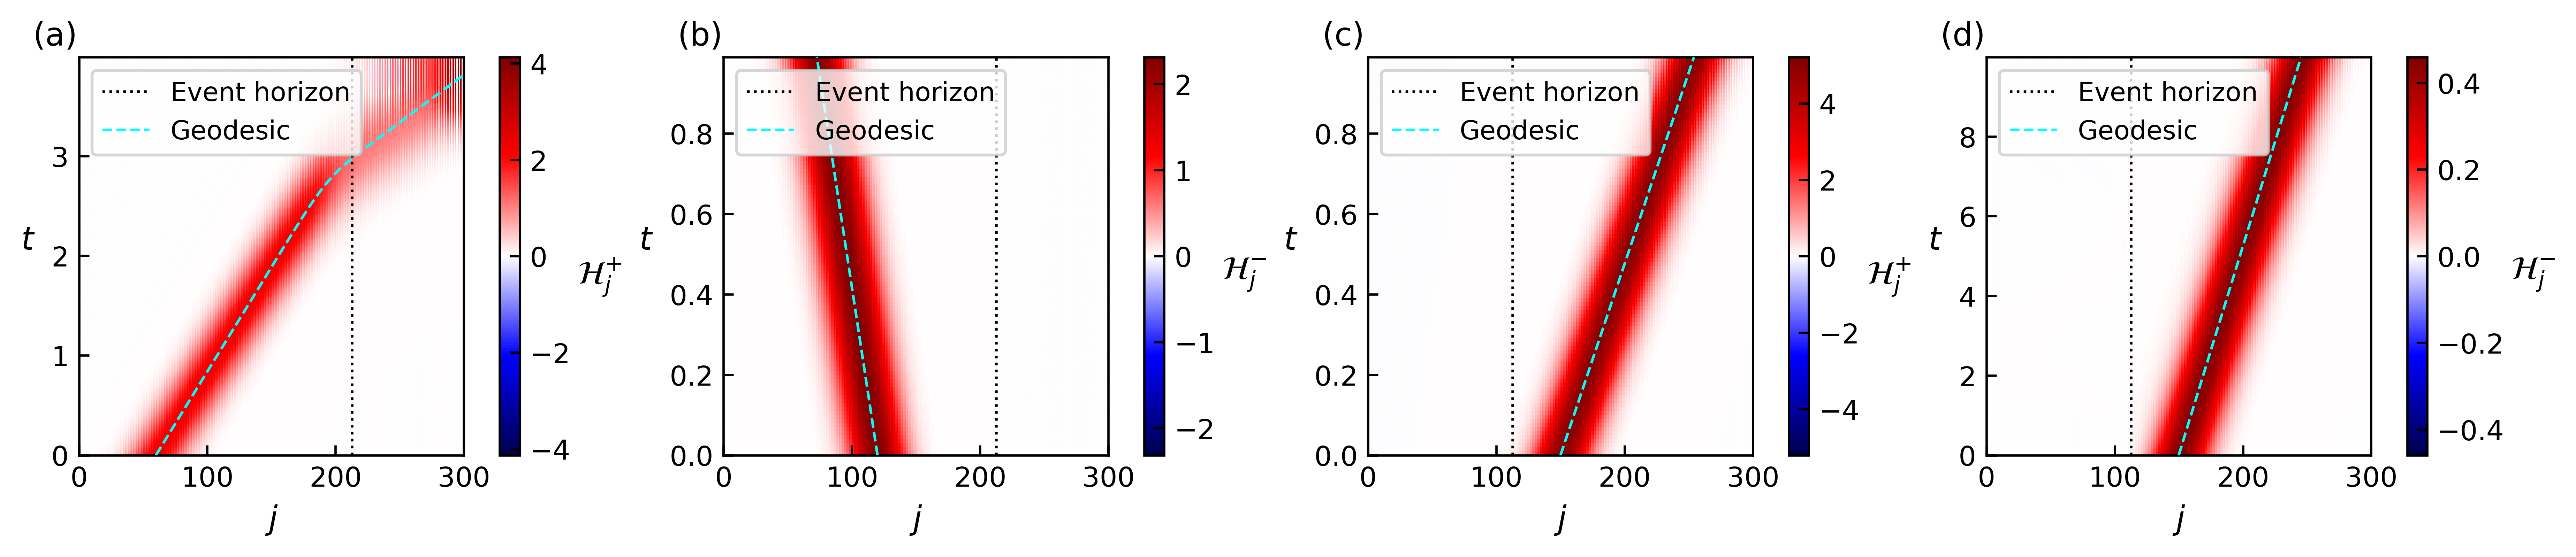
\includegraphics[width=\linewidth]{figure/p=0_BH.png}
\caption{Wave packet dynamics for the black-hole profile with $p=0$. The system parameters are $L=300$, $\ell=2\pi$, and $\beta(x)=A\tanh[B(x-x_0)]+C$ with $A=0.6$, $B=3$, and $C=0.6$. In (a,b), $x_0=2\ell/3$ and the event horizon is at $j_h\approx213$; in (c,d), $x_0=\ell/3$ and the event horizon is at $j_h\approx113$. (a) Packet initialized outside the horizon with ingoing group velocity ($j_0=60$, $\sigma=0.05L$). (b) Packet initialized outside the horizon with outgoing group velocity ($j_0=120$, $\sigma=0.05L$). (c) Packet initialized inside the horizon with a right-moving initial spinor ($j_0=150$, $\sigma=0.05L$). (d) Packet initialized inside the horizon with a left-moving initial spinor ($j_0=150$, $\sigma=0.05L$). The color scale shows the branch-resolved, vacuum-subtracted energy density $\delta\mathcal{E}_{j,+}$ in (a,c) and $\delta\mathcal{E}_{j,-}$ in (b,d) [Eq.~\eqref{eq:branch_resolved_energy}]. Black dotted lines indicate the event horizon, and cyan curves indicate the corresponding null geodesics $dx/dt=\beta(x)\pm1$.}
\label{fig:bh_p0}
\end{figure*}
We first examine the motion of the wave packet for the case $p=0$.
Fig.~\ref{fig:bh_p0} shows the time evolution of wave packets for several initial conditions.
The event horizon is indicated by the black dotted line, while the geodesic is shown by the light-blue curve.
The region to the right of the event horizon corresponds to the black-hole interior.
Figs.~\ref{fig:bh_p0}(a,b) show that wave packets initially placed outside the black hole follow the corresponding geodesic trajectories for both ingoing and outgoing motion.
Figs.~\ref{fig:bh_p0}(c,d) show the time evolution of a wave packet initially placed inside the black hole.
Inside the event horizon, both characteristic velocities are positive in this setup, so wave packets propagate only toward increasing $x$.
Thus, the wave packet is expected to propagate only to the right.
The numerical results show that both the right-moving mode in Fig.~\ref{fig:bh_p0}(c) and the left-moving mode in Fig.~\ref{fig:bh_p0}(d) propagate in the rightward direction.
The initial state was chosen with $j_0=150$, and the standard deviation was set to $\sigma=0.05L$.

\begin{figure*}[t]
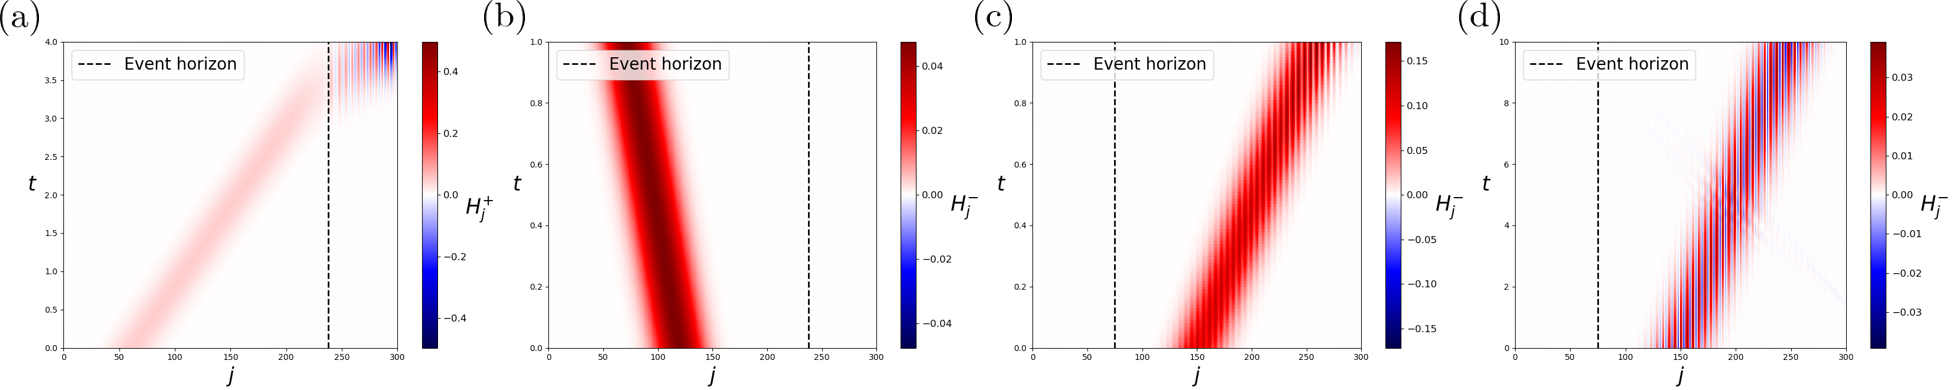
\includegraphics[width=\linewidth]{figure/p=1_BH.png}
\caption{Wave packet dynamics for the black-hole profile with $p=1$. System parameters are the same as in Fig.~\ref{fig:bh_p0}: in (a,b), $x_0=2\ell/3$ and $j_h\approx213$; in (c,d), $x_0=\ell/3$ and $j_h\approx113$. (a) Packet initialized outside the horizon with ingoing group velocity ($j_0=60$, $\sigma=0.05L$). (b) Packet initialized outside the horizon with outgoing group velocity ($j_0=120$, $\sigma=0.05L$). (c) Packet initialized inside the horizon with a right-moving initial spinor ($j_0=150$, $\sigma=0.05L$). (d) Packet initialized inside the horizon with a left-moving initial spinor ($j_0=150$, $\sigma=0.05L$). The color scale shows $\delta\mathcal{E}_{j,+}$ in (a,c) and $\delta\mathcal{E}_{j,-}$ in (b,d) [Eq.~\eqref{eq:branch_resolved_energy}]. Black dotted lines indicate the event horizon, and cyan curves indicate the corresponding null geodesics $dx/dt=\beta(x)\pm1$. Interior oscillations in (c,d) are more pronounced than in the $p=0$ case owing to the stronger excitation of doubler modes, as confirmed by the $k$-space analysis of Fig.~\ref{fig:doubler_fft}.}
\label{fig:bh_p1}
\end{figure*}
Next, we investigate the motion of the wave packet for the case $p=1$.
As in the case $p=0$, Figs.~\ref{fig:bh_p1}(a,b) show that wave packets initially placed outside the black hole follow the corresponding geodesic trajectories for both ingoing and outgoing motion.
Figs.~\ref{fig:bh_p1}(c,d) show that wave packets initially placed inside the black hole again propagate toward increasing $x$, as expected from the positive characteristic velocities inside the horizon.
Inside the black hole, the wave packet exhibits pronounced oscillatory behavior, whose origin can be traced to the doubler modes.
For the packet entering from the exterior [Fig.~\ref{fig:bh_p1}(a)], the oscillation develops after the packet reaches the interior.
This is caused by the excitation of doubler modes during time evolution.
Fig.~\ref{fig:doubler_fft}(a) shows the low-energy doubler modes that appear for $p=1$ inside the horizon, where $\beta>1$, while Fig.~\ref{fig:doubler_fft}(b) shows a secondary Fourier peak growing near the predicted wavenumber.
On the other hand, the oscillations in Figs.~\ref{fig:bh_p1}(c,d) are already present from the initial time.
Since these wave packets are initialized inside the black hole, they already have overlap with the doubler branch indicated in Fig.~\ref{fig:doubler_fft}(a).
Although the $p=0$ model also contains a doubler branch near $k=\pi$, the FFT analysis shows a larger doubler-mode peak for $p=1$ in the black-hole interior, explaining the more pronounced oscillations in Figs.~\ref{fig:bh_p1}(c,d).
\begin{figure*}[tbp]
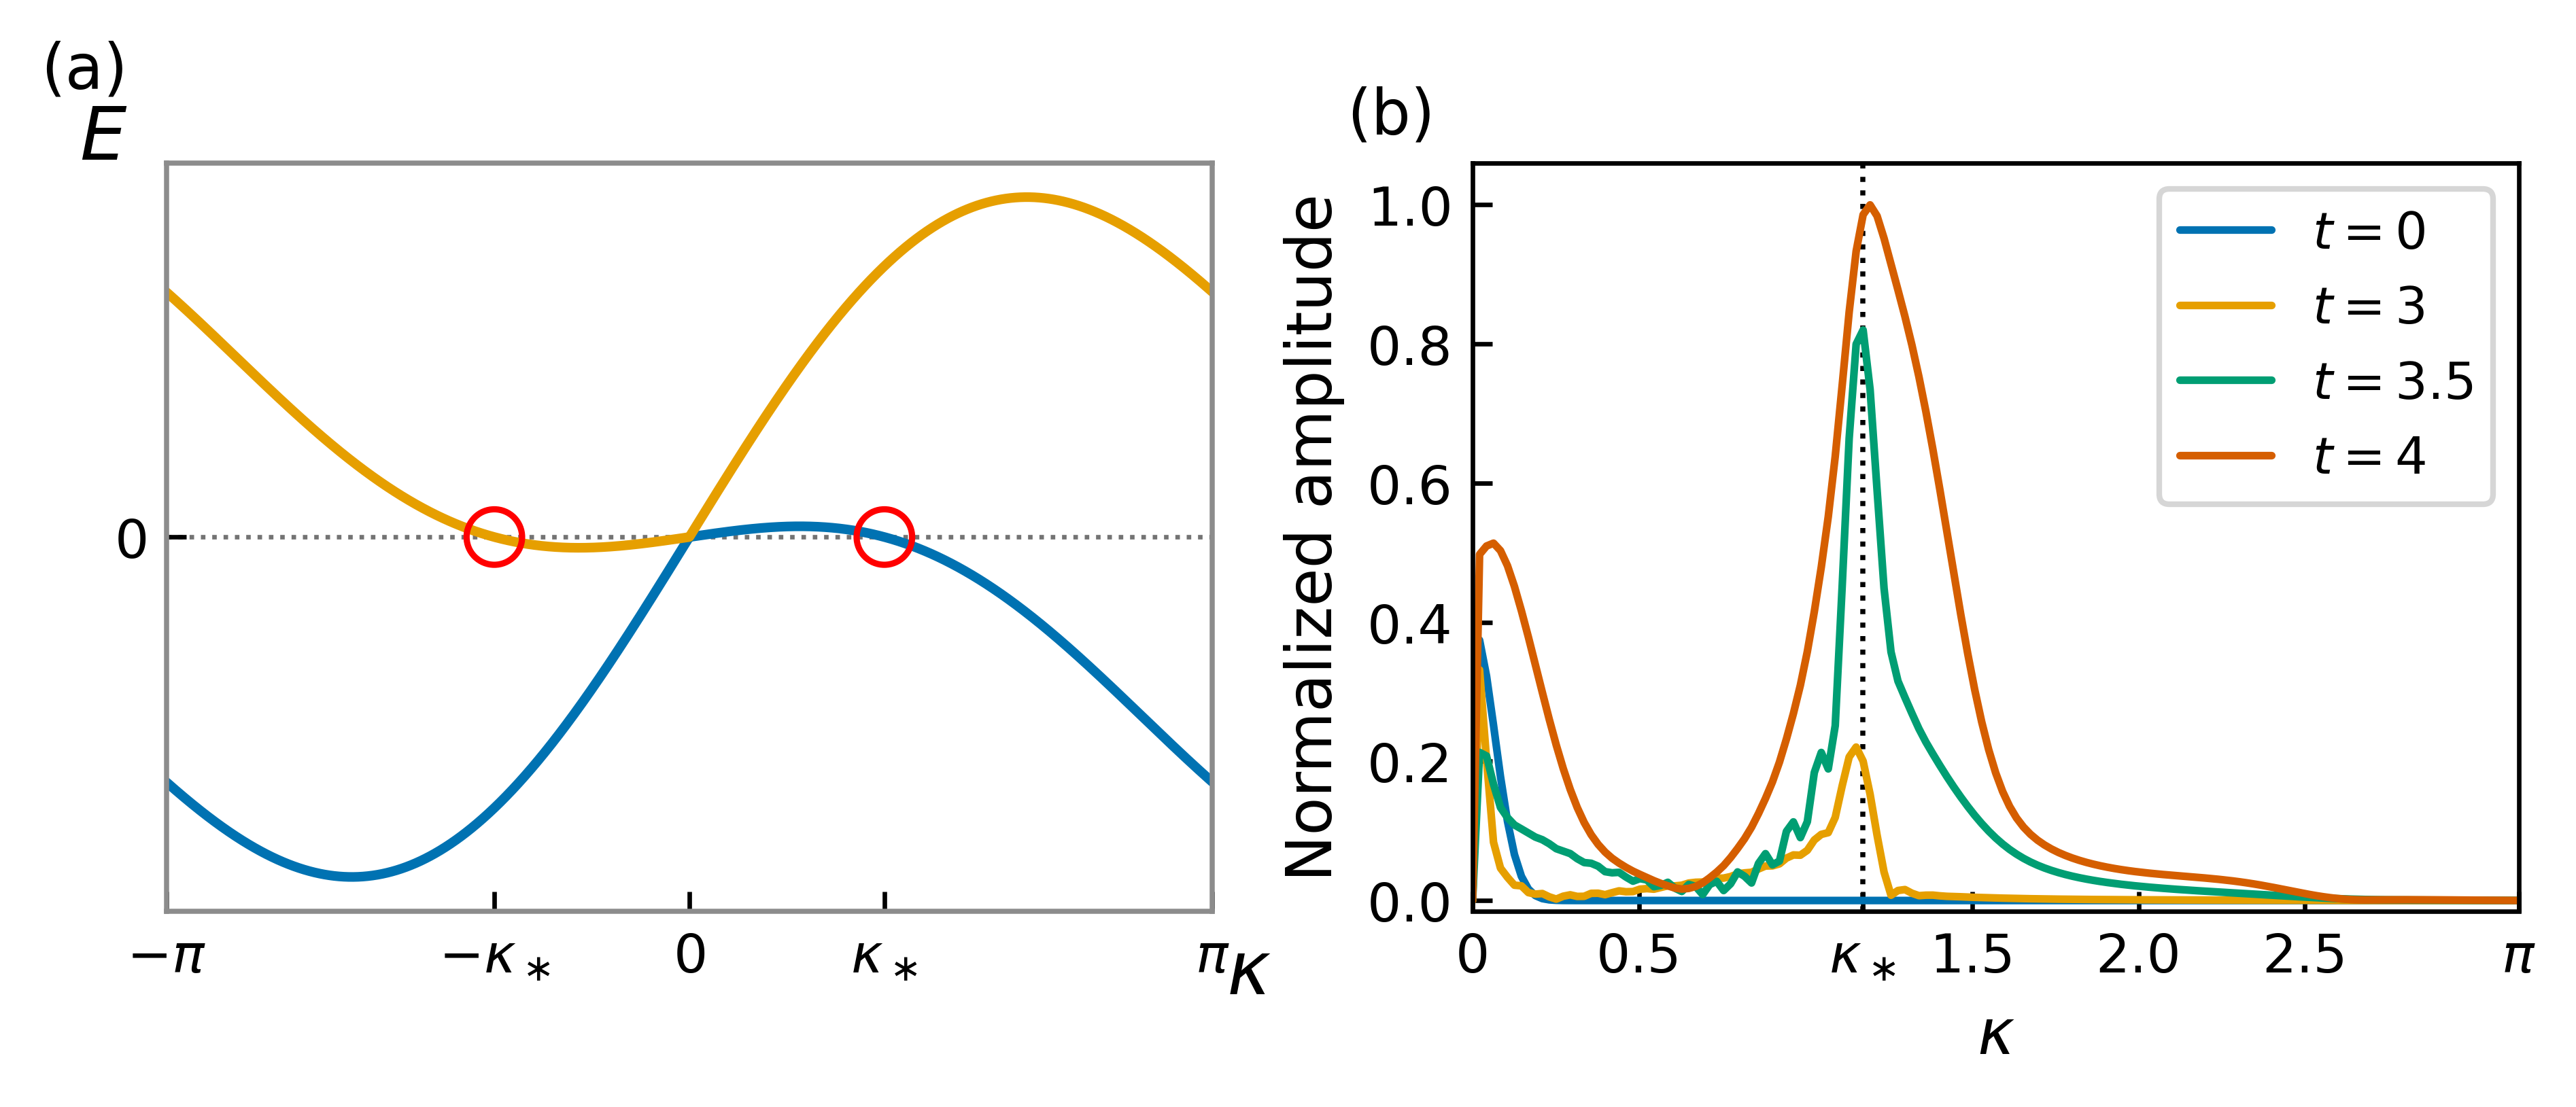
\includegraphics[width=\textwidth]{figure/doubler_fft.png}
\caption{Excitation of doubler modes in the oscillatory wave-packet dynamics for $p=1$.
(a) Local dispersion relation at $\beta=1.2$, representative of the black-hole interior.
The red circles mark the low-energy crossings at $k=\pm k_d$, corresponding to the doubler modes, where $k_d\simeq1.171$.
(b) Spatial FFT spectrum of the wave packet in Fig.~\ref{fig:bh_p1}(a) at successive times $t=0,3,3.5,4$, normalized by the maximum amplitude.
The black dotted line indicates the doubler-mode wave number $k_d$ predicted from (a).
The peak near $k=0$ corresponds to the low-momentum quasiparticle component, while the secondary peak grows near $k_d$ as the packet enters the black-hole interior.
This agreement supports the interpretation that the oscillatory behavior in Fig.~\ref{fig:bh_p1} originates from the excitation of doubler modes.}
\label{fig:doubler_fft}
\end{figure*}

We next extract the surface gravity of the effective horizon from the near-horizon wave-packet dynamics.
For a left-moving wave packet localized in the exterior region near the event horizon, the linearized near-horizon null-geodesic equation gives the approximate growth of the energy-density-weighted standard deviation defined in Eq.~\eqref{eq:energy_weighted_width},
\begin{align}
    \delta\sigma_{\mathcal E}(t) \propto e^{\kappa t}-1,
    \label{eq:sigma_kappa}
\end{align}
where $\kappa=|\beta'(x_h)|$ is the surface gravity.
This approximate relation follows by linearizing the left-moving null trajectory $dx/dt=\beta(x)-1$ near the horizon, where $\beta(x_h)=1$, giving $d(x-x_h)/dt\simeq\kappa(x-x_h)$ and hence exponential stretching of the wave packet.
It implies that the surface gravity can be read off from the exponential growth rate of $\delta\sigma_{\mathcal E}$ as long as the wave packet remains in the near-horizon regime.
In practice, we fit the numerical data to $a(e^{\kappa_{\rm fit}t}-1)$, where $a$ is a prefactor and $\kappa_{\rm fit}$ is the fitted growth rate.

For the surface-gravity extraction (Fig.~\ref{fig:sg}), we use $A=1$, $B=1$, $C=1$, $x_0=\pi$ (so $x_h=x_0$, $\kappa=|\beta'(x_h)|=1$, and $j_h=0.5L$), $j_0=245$, $\sigma=0.003L$, and fit the data over the time interval $t\in[0,1]$.
\begin{figure*}[tbp]
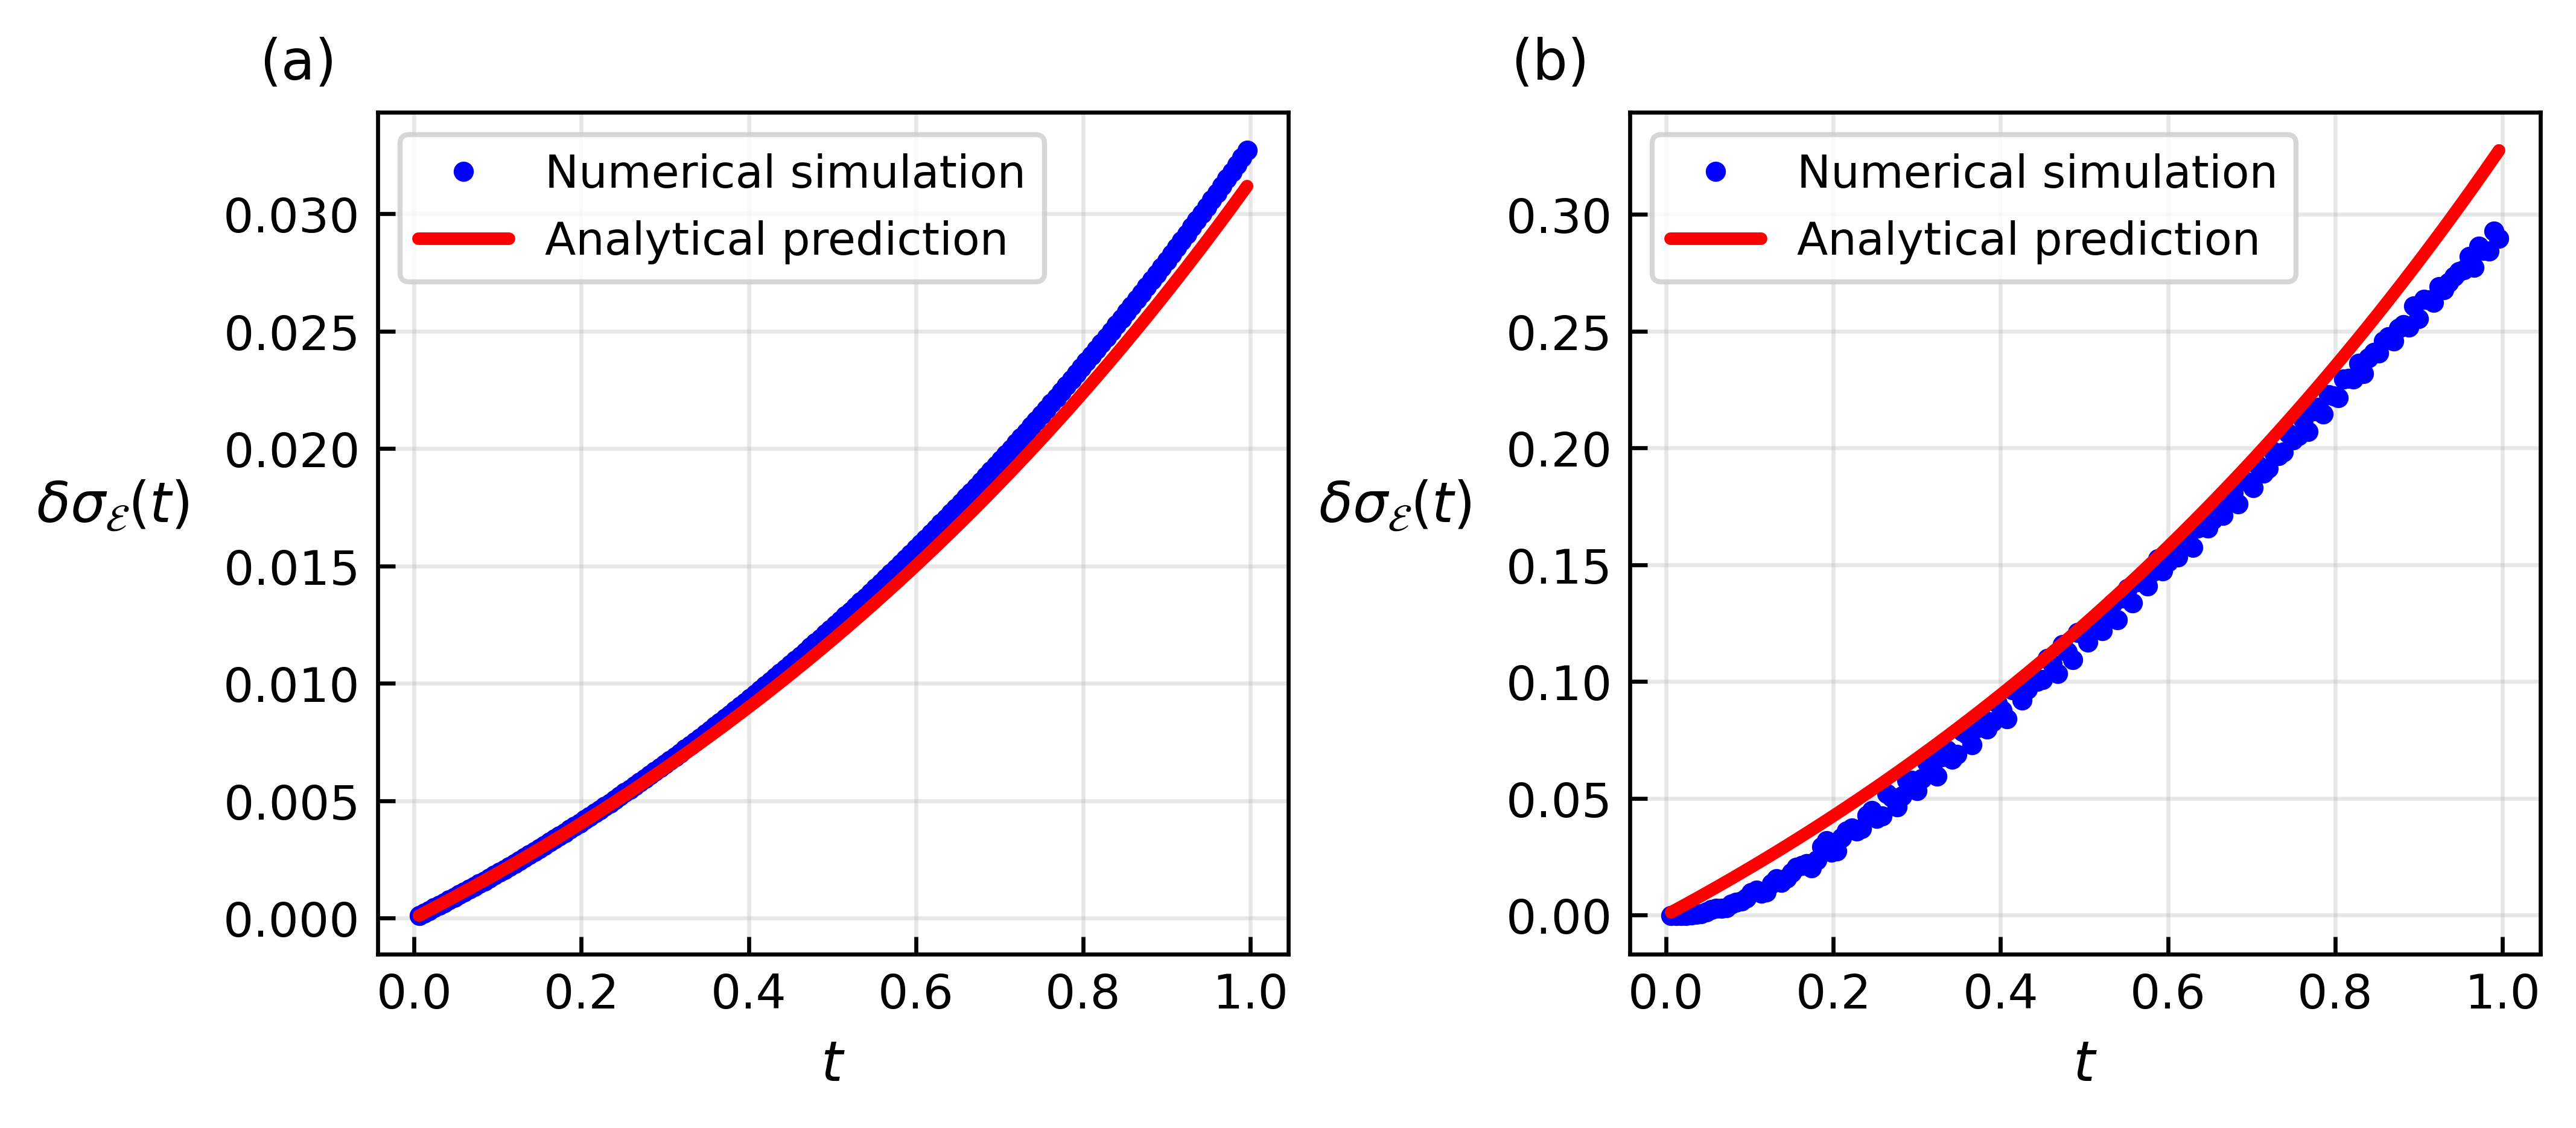
\includegraphics[width=\textwidth]{figure/sg.png}
\caption{Extraction of surface gravity from wave-packet broadening ($L=500$, $A=B=C=1$, $x_0=\ell /2$, $j_0=245$, $\sigma=0.003L$, with the fit performed over $t\in[0,1]$). Blue dots show the numerical energy-density-weighted width $\delta\sigma_{\mathcal E}(t)$ defined in Eq.~\eqref{eq:energy_weighted_width}, and red curves show the analytical near-horizon scaling $a(e^{\kappa t}-1)$ with $\kappa=1$; the prefactor $a$ fixes the vertical scale. The fitted growth rates are obtained separately from $a(e^{\kappa_{\rm fit}t}-1)$. (a) Result for $p=0$, with $|\kappa_{\rm fit}-\kappa|/\kappa\approx3.3\%$. (b) Result for $p=1$, with $|\kappa_{\rm fit}-\kappa|/\kappa\approx4.9\%$ due to simultaneous wave packet dispersion. These percentages quantify the error in the fitted surface gravity, not the pointwise deviation of the red analytical curves.}
\label{fig:sg}
\end{figure*}
Fig.~\ref{fig:sg} compares the numerical data with the analytical near-horizon form for $\kappa=1$, while the quoted $\kappa_{\rm fit}$ values are obtained by allowing the exponential growth rate to vary.
As shown in Fig.~\ref{fig:sg}(a), for $p=0$, the fitted growth rate agrees with the analytical surface gravity $\kappa=1$ within a relative error of approximately 3.3\%.
Small deviations from the analytical near-horizon curve at later times can be attributed to the breakdown of the approximation in Eq.~\eqref{eq:sigma_kappa} as the wave packet moves away from the event horizon.

In contrast, for $p=1$, the discrepancy is larger than in the $p=0$ case.
The relative error of the fitted growth rate with respect to the analytical value is about 4.9\%.
This discrepancy can be attributed to deformation of the wave packet as it broadens, which causes deviations from the simple exponential behavior.

\subsection{White Hole}
In this section, we present the results of numerical simulations of particle dynamics in a white-hole spacetime. We consider the case in which a wave packet is incident from the exterior toward the interior of the white hole. We also discuss the finite-size effects that arise in this setup.
For the white-hole dynamics, we use $A=C=-0.6$, $B=3$, $x_0=2\ell/3$ (white-hole horizon at $j_h\approx213$ for $L=300$), with $j_0=0.2L$ and $\sigma=0.05L$.
\begin{figure*}[tbp]
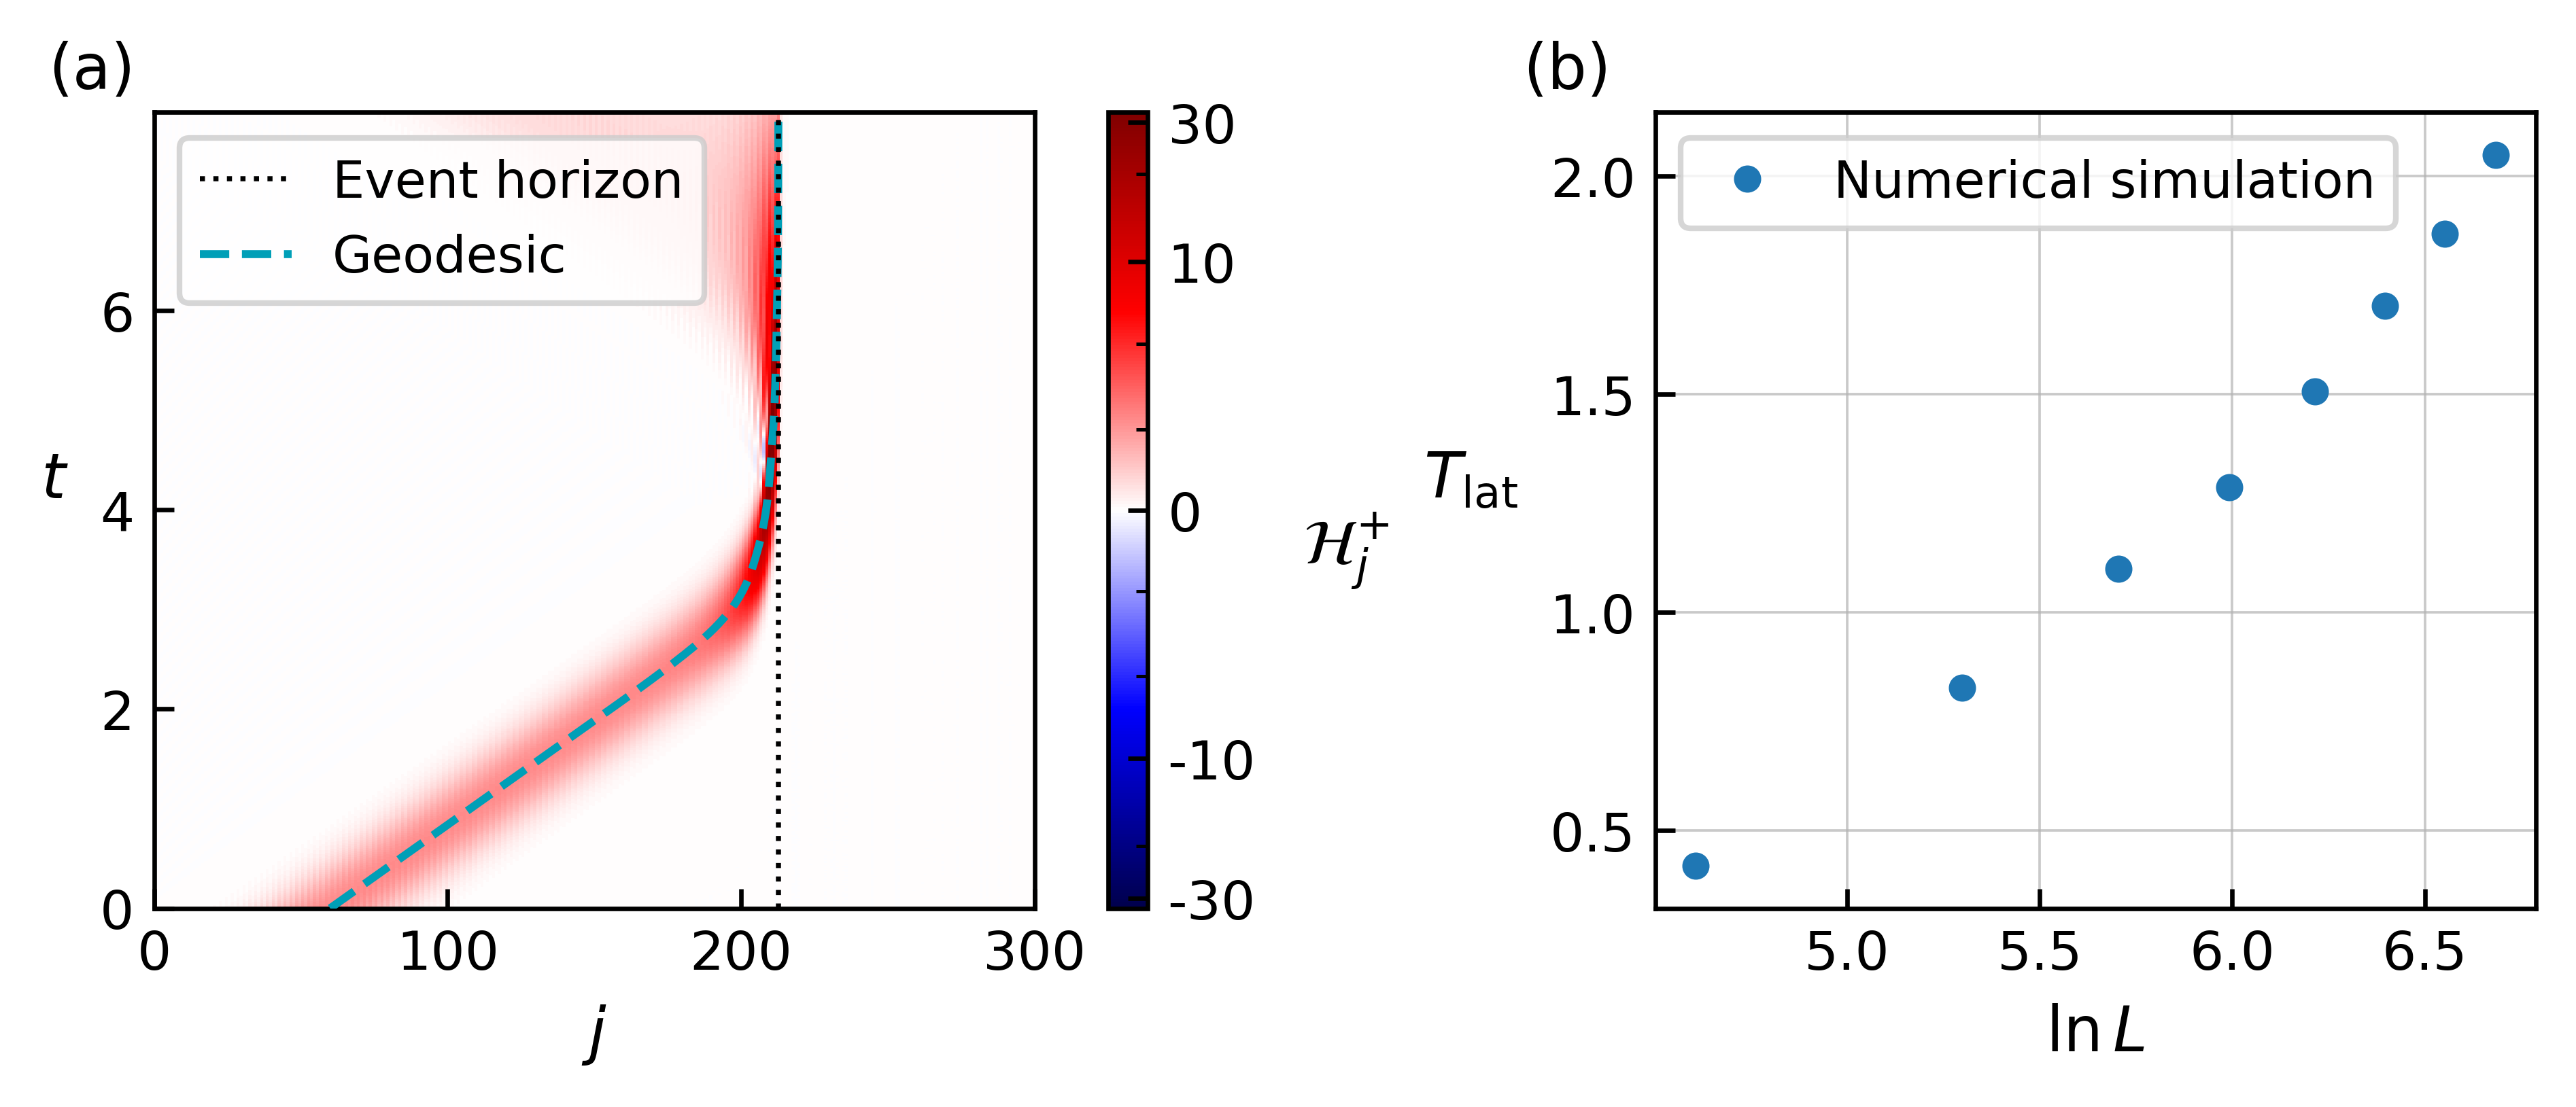
\includegraphics[width=\textwidth]{figure/WH_p=0.png}
\caption{Wave packet dynamics in the white-hole geometry for $p=0$. (a) Space-time diagram of the vacuum-subtracted energy density $\delta\mathcal{E}_{j,+}$ [Eq.~\eqref{eq:branch_resolved_energy}] for $L=300$, $j_0=0.2L$, and $\sigma=0.05L$, with $\beta$ profile parameters $A=C=-0.6$, $B=3$, and $x_0=2\ell/3$ (white-hole horizon at $j_h\approx213$). The wave packet is compressed toward the white-hole horizon (black dotted line) and eventually reflected due to finite lattice resolution. (b) Lattice stagnation time $T_{\mathrm{lat}}$ versus $\ln L$ for various system sizes, using $A=C=-0.6$, $B=3$, $x_0=2\ell/3$, $j_0=0.2L$, and $\sigma=0.05L$. Blue dots show numerical simulation results; their approximately linear dependence on $\ln L$ is consistent with the logarithmic scaling of Eq.~\eqref{eq:T_logL}.}
\label{fig:wh_p0}
\end{figure*}
For $p = 0$, as shown in Fig.~\ref{fig:wh_p0}, the wave packet is initially compressed at the white-hole horizon, yielding behavior consistent with the ideal analytical expectation. However, after a certain time, the wave packet collapses and is reflected. This behavior is attributed to a finite-size effect arising when the wave-packet standard deviation becomes smaller than the lattice spacing.
For the stagnation-time scaling in Fig.~\ref{fig:wh_p0}(b), we use the same profile parameters, $A=C=-0.6$, $B=3$, and $x_0=2\ell/3$, with $j_0=0.2L$ and $\sigma=0.05L$.
Near the white-hole horizon, the same linearized null-geodesic argument gives an exponential compression of the wave-packet standard deviation, $\sigma(t)\propto\sigma_0 e^{-\kappa t}$.
In the lattice model, this continuum description breaks down once this standard deviation becomes comparable to the lattice spacing $\varepsilon=\ell/L$.
Defining the continuum estimate of the stagnation time $T_{\mathrm{cont}}$ by $\sigma(T_{\mathrm{cont}})\sim\varepsilon$, one obtains
\begin{align}
    T_{\mathrm{cont}} \propto \ln L ,
    \label{eq:T_logL}
\end{align}
for fixed continuum size $\ell$ and fixed initial physical standard deviation $\sigma_0$.

We then test this logarithmic scaling by examining the dependence of the lattice stagnation time $T_{\mathrm{lat}}$ on the system size $L$.
To define $T_{\mathrm{lat}}$ in the numerical data, we identify an onset time $t_{\mathrm{in}}$ for the compression regime.
Operationally, after the wave packet has entered the compression stage, $t_{\mathrm{in}}$ is taken as the first time at which
$|\partial_x^2\beta(\bar{x}(t))|<0.1$, where $\bar{x}(t)$ is the wave-packet mean position.
We then identify the time $t_{\mathrm{min}}$ at which the wave-packet standard deviation reaches its minimum.
The lattice stagnation time is then defined operationally as $T_{\mathrm{lat}} = t_{\mathrm{min}} - t_{\mathrm{in}}$.
The approximately linear dependence of the data on $\ln L$ in Fig.~\ref{fig:wh_p0}(b) is consistent with the logarithmic system-size scaling predicted for $T_{\mathrm{cont}}$.
This comparison tests only the logarithmic dependence, not its coefficient: $T_{\mathrm{lat}}$ is defined operationally from the nonlinear lattice collapse and reflection, so its slope need not equal the continuum value $1/\kappa$.
Therefore, we conclude that the reflection of the wave packet is caused by a finite-size effect associated with its standard deviation becoming smaller than the lattice spacing.

\begin{figure*}[tbp]
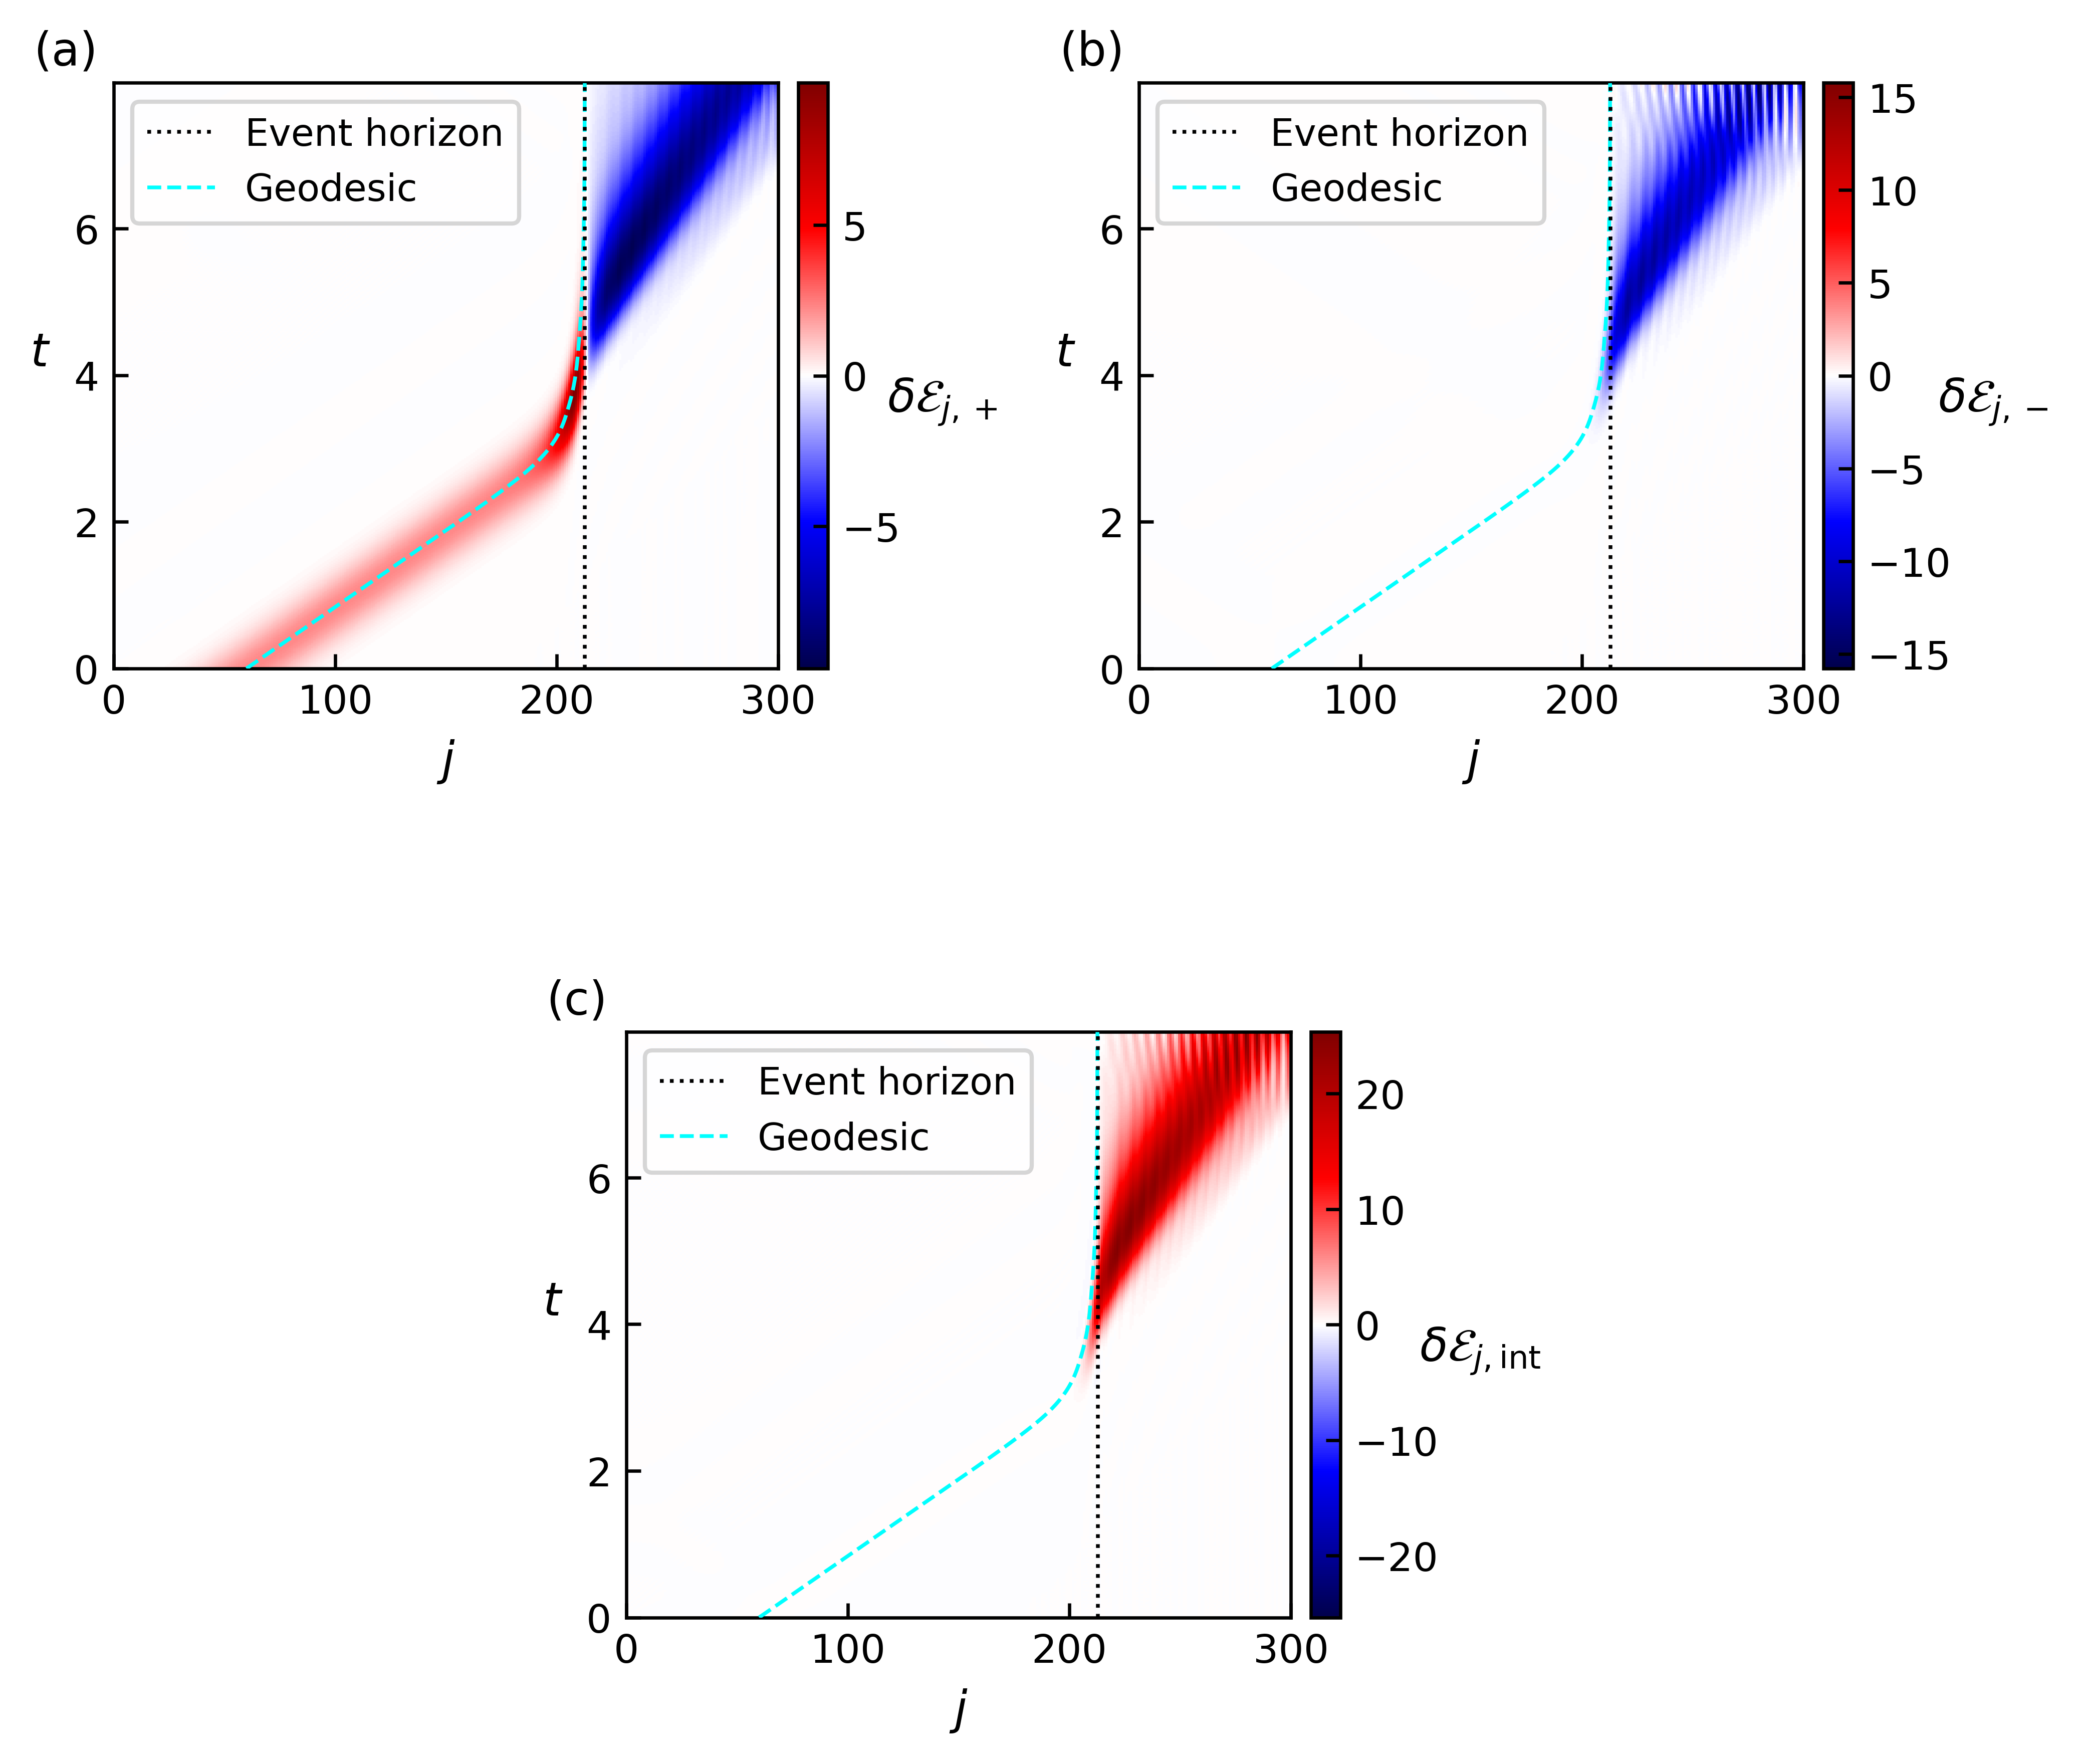
\includegraphics[width=\textwidth]{figure/WH_p=1.png}
\caption{White-hole dynamics for $p=1$ ($L=300$, $j_0=0.2L$, $\sigma=0.05L$, with the same $\beta$ profile as Fig.~\ref{fig:wh_p0}(a), $A=C=-0.6$, $B=3$, $x_0=2\ell/3$, and $j_h\approx213$). (a) Space-time diagram of the vacuum-subtracted energy density $\delta\mathcal{E}_{j,+}$. (b) Space-time diagram of $\delta\mathcal{E}_{j,-}$. (c) Space-time diagram of the mixed contribution $\delta\mathcal{E}_{j,\mathrm{int}}$ built from $\mathcal{H}_j^{\mathrm{int}}$. Unlike the $p=0$ case, the coupling between the right- and left-moving components allows partial transmission across the white-hole horizon (black dotted line).}
\label{fig:wh_p1}
\end{figure*}
For $p=1$, the wave-packet dynamics differs from the $p=0$ case.
As shown in Fig.~\ref{fig:wh_p1}, part of the wave packet crosses the white-hole horizon instead of being simply reflected.
This behavior is absent for $p=0$, indicating that the coupling between the right- and left-moving modes plays an important role.

\section{CONCLUSIONS}
In this work, we have investigated particle dynamics in a one-dimensional lattice fermion model designed to simulate black-hole and white-hole spacetimes, focusing on the correspondence between lattice wave-packet trajectories and geodesics of the effective curved metric.

For the black-hole geometry, Gaussian wave packets initialized both outside and inside the event horizon closely follow the corresponding geodesics for both $p=0$ and $p=1$ parameter choices. The oscillatory behavior observed inside the black hole arises from doubler modes, with the $p=1$ case exhibiting more pronounced oscillations owing to stronger overlap with, and excitation of, these modes. We also extracted the surface gravity from the exponential growth of the wave-packet standard deviation in the near-horizon regime, finding agreement within a relative error of $\sim 3.3\%$ for $p=0$ and a larger discrepancy of $\sim 4.9\%$ for $p=1$, with the latter attributed to deformation of the wave packet during broadening.

For the white-hole geometry, the wave packet is compressed toward the white-hole horizon in a manner consistent with the continuum expectation, but eventually collapses and reflects due to a finite-size effect. The lattice stagnation time is consistent with the logarithmic system-size scaling $T_{\mathrm{lat}}\propto\ln L$. For $p=1$, partial transmission across the white-hole horizon is observed, indicating that the coupling between left- and right-moving modes plays an important role.

These results demonstrate that the one-dimensional lattice fermion model provides a controlled setting for assessing curved-spacetime particle dynamics in lattice fermion simulators. Future directions include extending the model to dynamical black-hole backgrounds to investigate Hawking radiation from time-dependent horizons, as well as implementing the lattice Hamiltonian on near-term quantum hardware to experimentally probe this effect.

\bibliography{books}

\end{document}
